\chapter{Results}
% \section{Preprocessing Comparisons}
% Several preprocessing methods were applied and compared across the two datasets used in this study. The \textit{House Prices} dataset, available from this \href{https://www.kaggle.com/competitions/house-prices-advanced-regression-techniques/data}{Kaggle link}, contains various features about houses and their prices, while the \textit{Iris} dataset provides measurements of iris flowers across different species.\\
% This study evaluated the preprocessing capabilities of the Qwen2.5 language model by applying it to two distinct datasets: the \textit{Iris} dataset, which contains exclusively numerical data, and the \textit{House Prices} dataset, which includes both numerical and categorical features. The primary objective was to identify the optimal preprocessing steps suggested by Qwen2.5 for each dataset.

\section{Preprocessing Comparisons}
This study compared several preprocessing methods across two datasets: the
\textit{House Prices} dataset from Kaggle, which includes various features
related to houses and their prices, and the \textit{Iris} dataset, which
contains measurements of iris flowers from different species. \\ The focus was
on evaluating the preprocessing capabilities of the Qwen2.5 language model. It
was applied to both datasets: \textit{Iris}, which is purely numerical, and
\href{https://www.kaggle.com/competitions/house-prices-advanced-regression-techniques/data}{\textit{House
        Prices}}, which features both numerical and categorical data. The goal was to
identify the most effective preprocessing steps for each dataset as suggested
by Qwen2.5.

After extensive testing, the best preprocessing outcomes generated by Qwen2.5
were selected. These results were then benchmarked against two established
preprocessing approaches:

\begin{enumerate}
    \item Preprocessing steps performed by our team and the Kaggle's users, specifically
          those rated as high-quality for each dataset.
    \item A parallel experiment using the LLaMA language model, in which identical
          preprocessing objectives and criteria were applied to ensure a fair comparison.
\end{enumerate}

The comparative analysis focused on multiple dimensions of preprocessing
performance, including the alignment of recommended steps with best practices,
the efficiency of data preparation, and the comprehensiveness in handling
missing values, scaling, encoding, and feature engineering. Additionally,
similarities and differences in the preprocessing pipelines across Qwen2.5,
Kaggle benchmarks, and the LLaMA model were examined to assess each model's
compatibility with established standards and adaptability to datasets with both
numerical and categorical features.

This section presents the findings from these comparisons, highlighting the
consistency, robustness, and adaptability of the preprocessing steps suggested
by Qwen2.5, relative to those obtained from experienced Kaggle practitioners
and the LLaMA model.

\subsection{House Prices Dataset}

\subsubsection{Comparison 1: Preprocessing by our Team}

The first step in preprocessing the \textit{House Prices} dataset involved
loading the dataset and examining its structure, which included analyzing the
features, data types, and missing values. This examination provided a clear
understanding of the data and informed the necessary steps for cleaning and
transformation.

The Id column was identified as irrelevant for the prediction model and was
removed from both the training and test datasets. The dataset was then split
into two parts: XX, representing the input features (excluding the target
variable, \textit{SalePrice}), and yy, the target variable \textit{SalePrice}.
Upon inspection, no duplicate rows were found, and therefore no action was
taken to remove any.

Outliers were identified through visual inspection by plotting
\textit{SalePrice} against \textit{GrLivArea}. Five extreme outliers were
detected and subsequently removed from the dataset to prevent distortion in the
model's performance.

Next, missing values in the numerical columns were addressed by imputing them
with the median value of the respective columns, ensuring no data were lost.
For some ordinal columns, where there were several unique values, similar
categories were grouped together to simplify the data and reduce complexity.

New columns were created by combining existing ones to reduce dimensionality
and potentially enhance the predictive power of the model. Only the most
relevant features, as determined by a correlation matrix, were retained for
further analysis.

Categorical columns were then encoded using One-Hot Encoding, ensuring they
were transformed into a numerical format suitable for machine learning
algorithms. Finally, numerical columns were scaled using the StandardScaler
method to standardize the features and ensure all variables were on the same
scale, facilitating better model convergence and performance.

\subsubsection{Comparison 2: Preprocessing by Alexandru Papiu}

Alexandru Papiu, a Kaggle user, applied preprocessing steps to the
\textit{House Prices} dataset. The notebook can be found in this
\href{https://www.kaggle.com/code/apapiu/regularized-linear-models}{Kaggle
    link}.

In order to make the distribution of skewed features more "normal" (selecting
those with skew > 0.75) the target variable (SalePrice) is transformed to
reduce skewness and make it more normally distributed using a log
transformation.

Then, dummy variables are created for categorical features using to transforms
categorical data into a format suitable for machine learning algorithms, where
each unique category becomes a separate binary feature.

After this, numeric features with missing values (NaN) are replaced with the
mean of their respective columns. This step ensures that no data points are
missing and that all columns have valid values for subsequent modeling.

Before and after transformations, histograms are plotted to visualize the
effect of the log transformation on SalePrice. This step helps demonstrate how
the transformation makes the distribution more normal.

The combined dataset is split back into training and testing feature sets. The
target variable (y) is extracted as the transformed SalePrice. This step
prepares the data for input into a machine learning model.

\subsubsection{Comparison 3: Preprocessing by Erik Bruin}

Another Kaggle user, Erik Bruin, has done preprocessing on the \textit{House
    Prices Dataset} at the following
\href{https://www.kaggle.com/code/erikbruin/house-prices-lasso-xgboost-and-a-detailed-eda}{kaggle
    link}.

The code first identifies columns with missing values (NA) and counts the
number of NAs for each column. This step allows a clear understanding of where
data is missing and how extensive the issue is.

The code works through the 34 predictors with missing values, starting from the
ones with the most NAs and addressing each systematically. Related variables
(e.g., Pool, Garage, Basement) are handled together when they form logical
groups.

Remaining character variables (non-numeric) are identified and processed. If
there is a clear order or hierarchy (ordinal data), they are encoded as ordinal
integers.

Where appropriate, variables are label-encoded or converted into one-hot
encoded features to prepare them for machine learning models.

Ordinal values are encoded using an ordinal scale for consistent ordering.

All NA values are filled or handled, ensuring complete data. Character and
numeric variables are converted into appropriate formats (factors, label
encoding, etc.) for further analysis.

Categorical variables are properly encoded for machine learning algorithms.

\subsubsection{Comparison 4: Automation of Data Preprocessing with LLaMA}

In this test, the LLaMA (version 3.2-Vision:11b) model was used to automate the
data preprocessing workflow. The task involved providing an unprocessed input
dataset and instructing LLaMA to generate a Python script that would perform
basic preprocessing tasks such as data cleaning, normalization, and encoding of
categorical variables.

Two specific prompts were used to guide LLaMA's output. The first (Level 1)
instructed LLaMA to analyze the dataset descriptor and identify necessary
preprocessing steps. The second (Level 2) asked LLaMA to generate Python code
to perform these preprocessing operations directly on the dataset.

Although LLaMA generated Python code based on these prompts, the resulting
script contained several errors and required human intervention to correct.
Some preprocessing steps also needed refinement for optimal performance.
Despite these challenges, the test demonstrated LLaMA's potential in automating
certain preprocessing tasks, though human oversight remained essential to
ensure the final script met the required standards.

\begin{figure}[H] 
    \centering 
    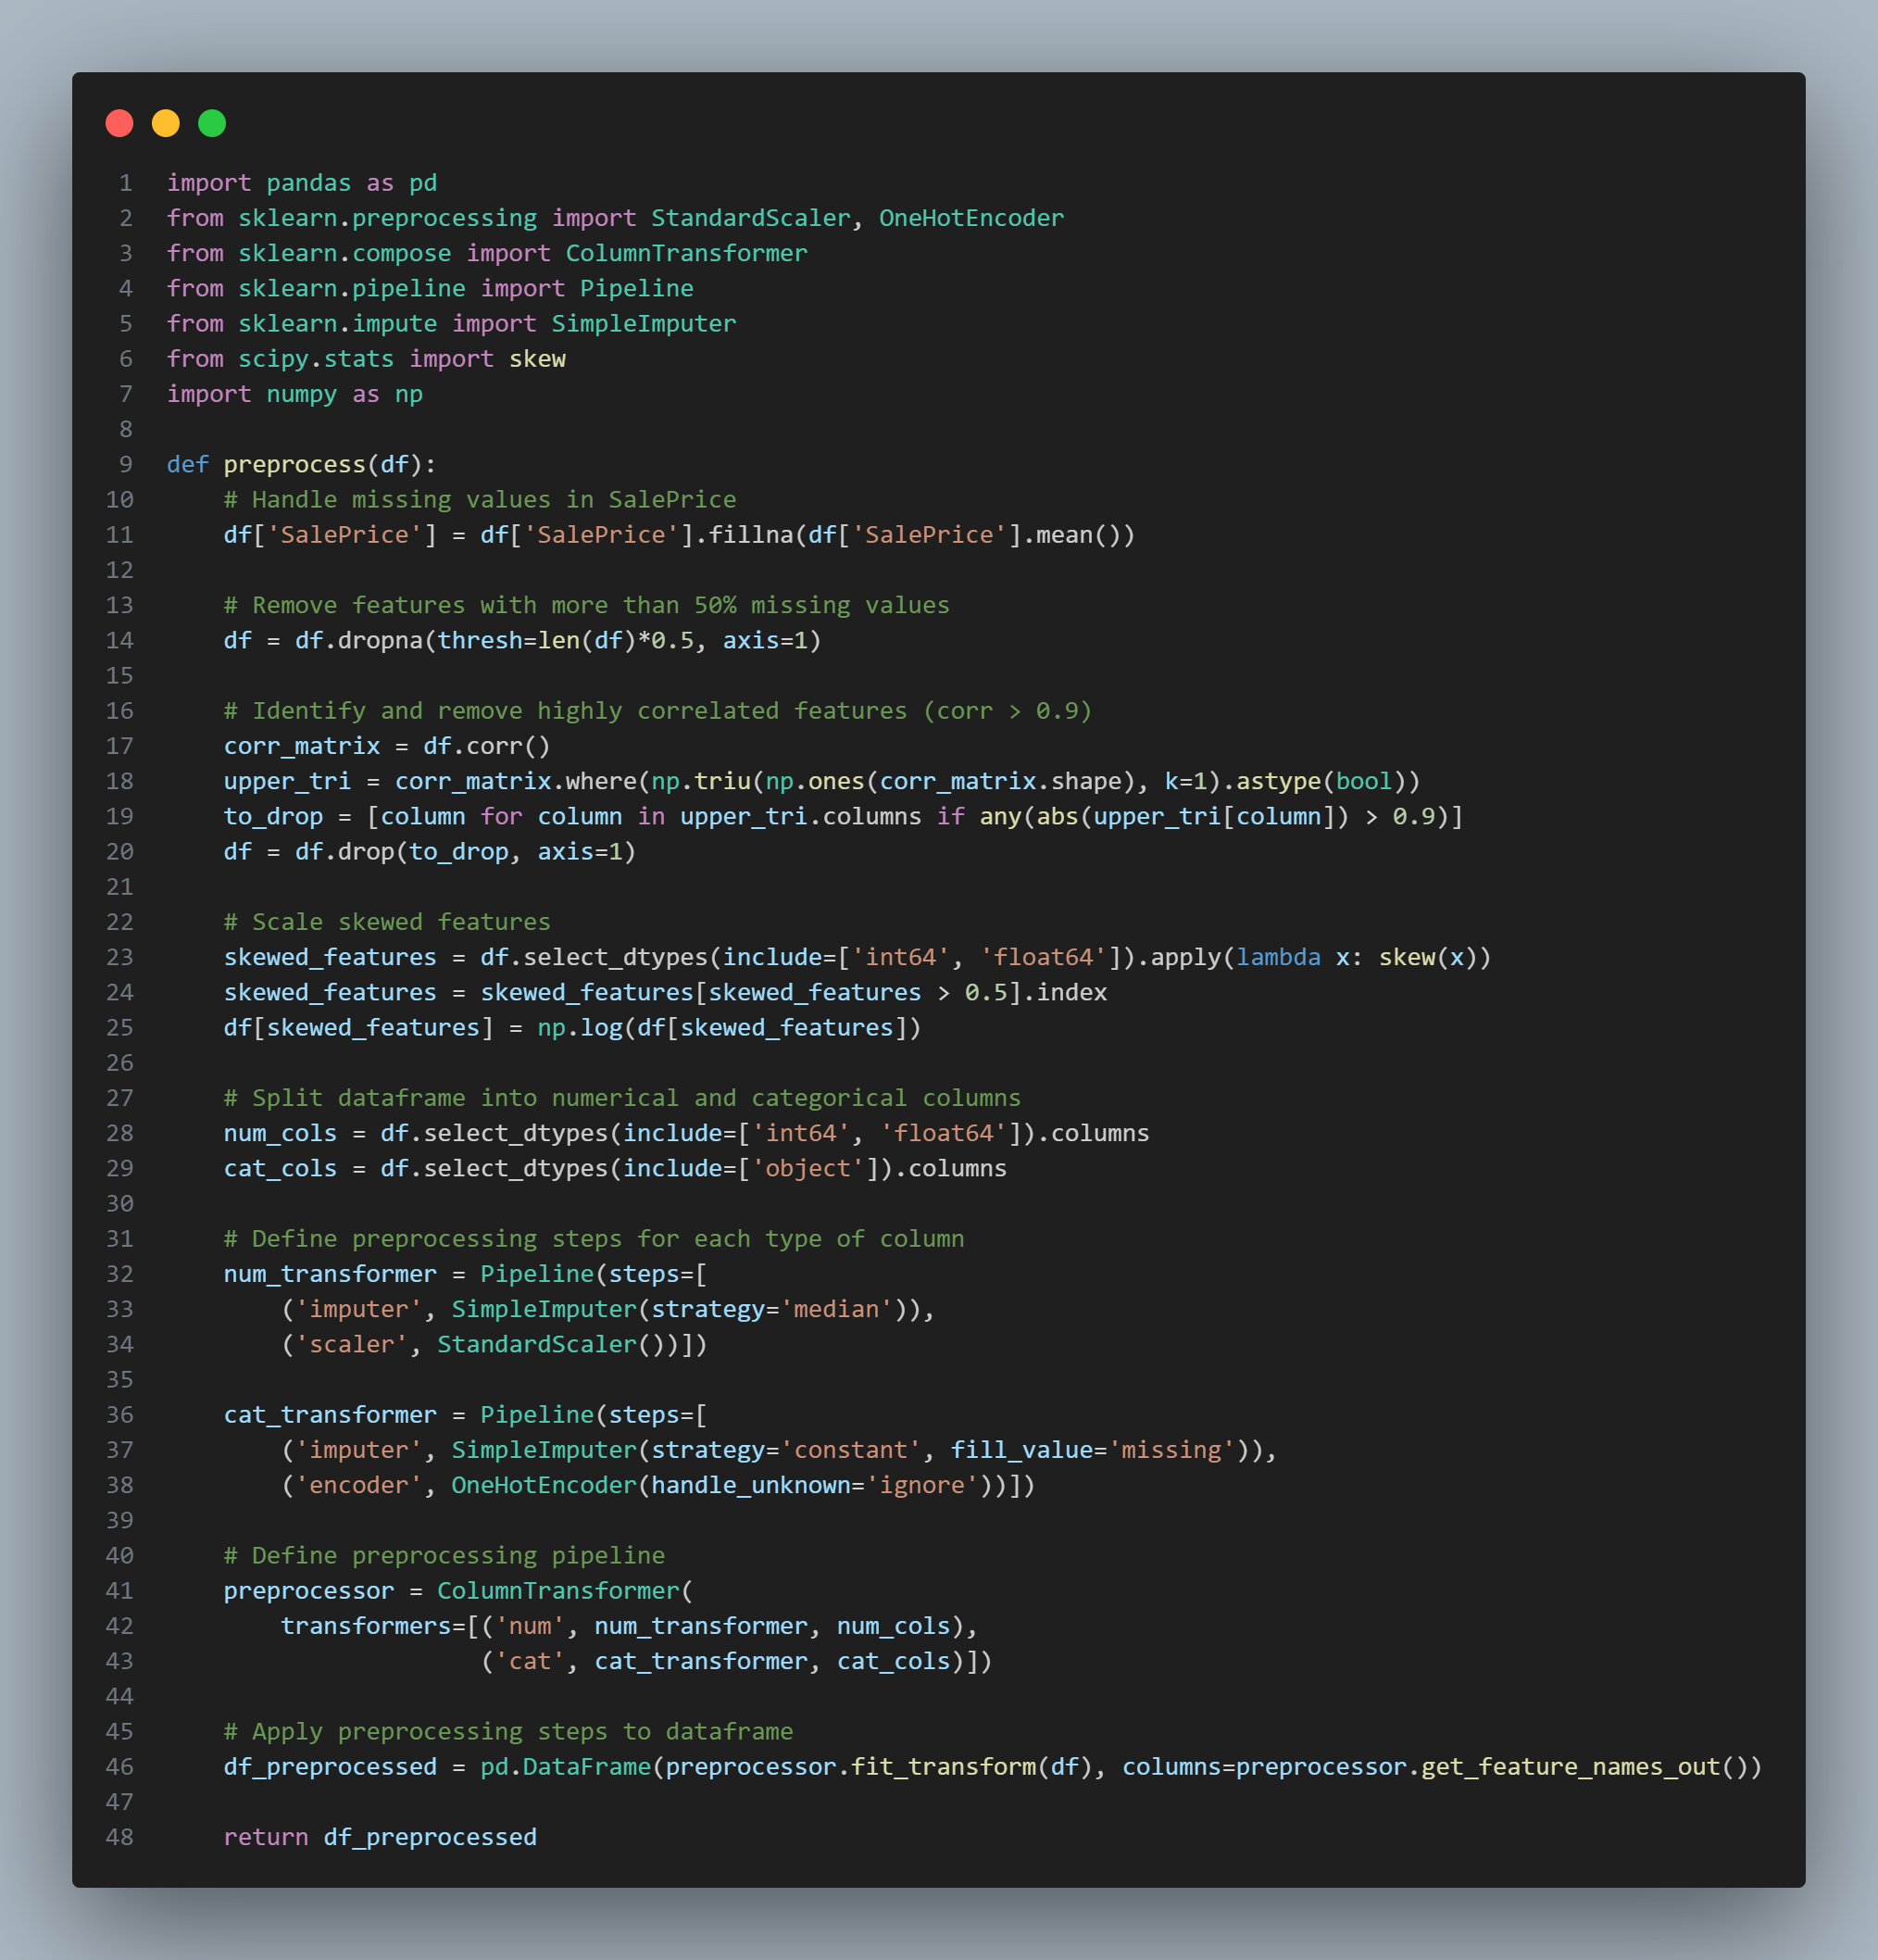
\includegraphics[width=0.7\textwidth]{media/LlamaCode.png} 
    \caption{Example of preprocessing script generated by LLaMA} 
\end{figure}

The use of \textit{role prompting} or \textit{persona prompting} in the
prompts, such as \textit{"You are a data engineer skilled in artificial
    intelligence..."} was particularly effective. This approach guides the LLM to
assume a professional role, focusing on the relevant aspects of the task and
tailoring responses to suit the context. This method helped in generating more
focused, accurate responses, minimizing ambiguity, and optimizing the overall
efficiency of the generated code.

\subsubsection{Our Approach: Application-Driven Preprocessing by Qwen2.5}

Multiple trials were run with varying prompts to assess the model's
effectiveness under different conditions. While the results showed promise,
they were slightly behind those achieved through other technologies or manual
methods, requiring several attempts to get acceptable performance.

Although still in development and dependent on current computational resources,
the application demonstrated clear potential for future improvement. While the
results were not perfect, they were encouraging, indicating that with
advancements in computational power and algorithm optimization, performance and
efficiency could be significantly enhanced.

\begin{figure}[H]
    \centering
    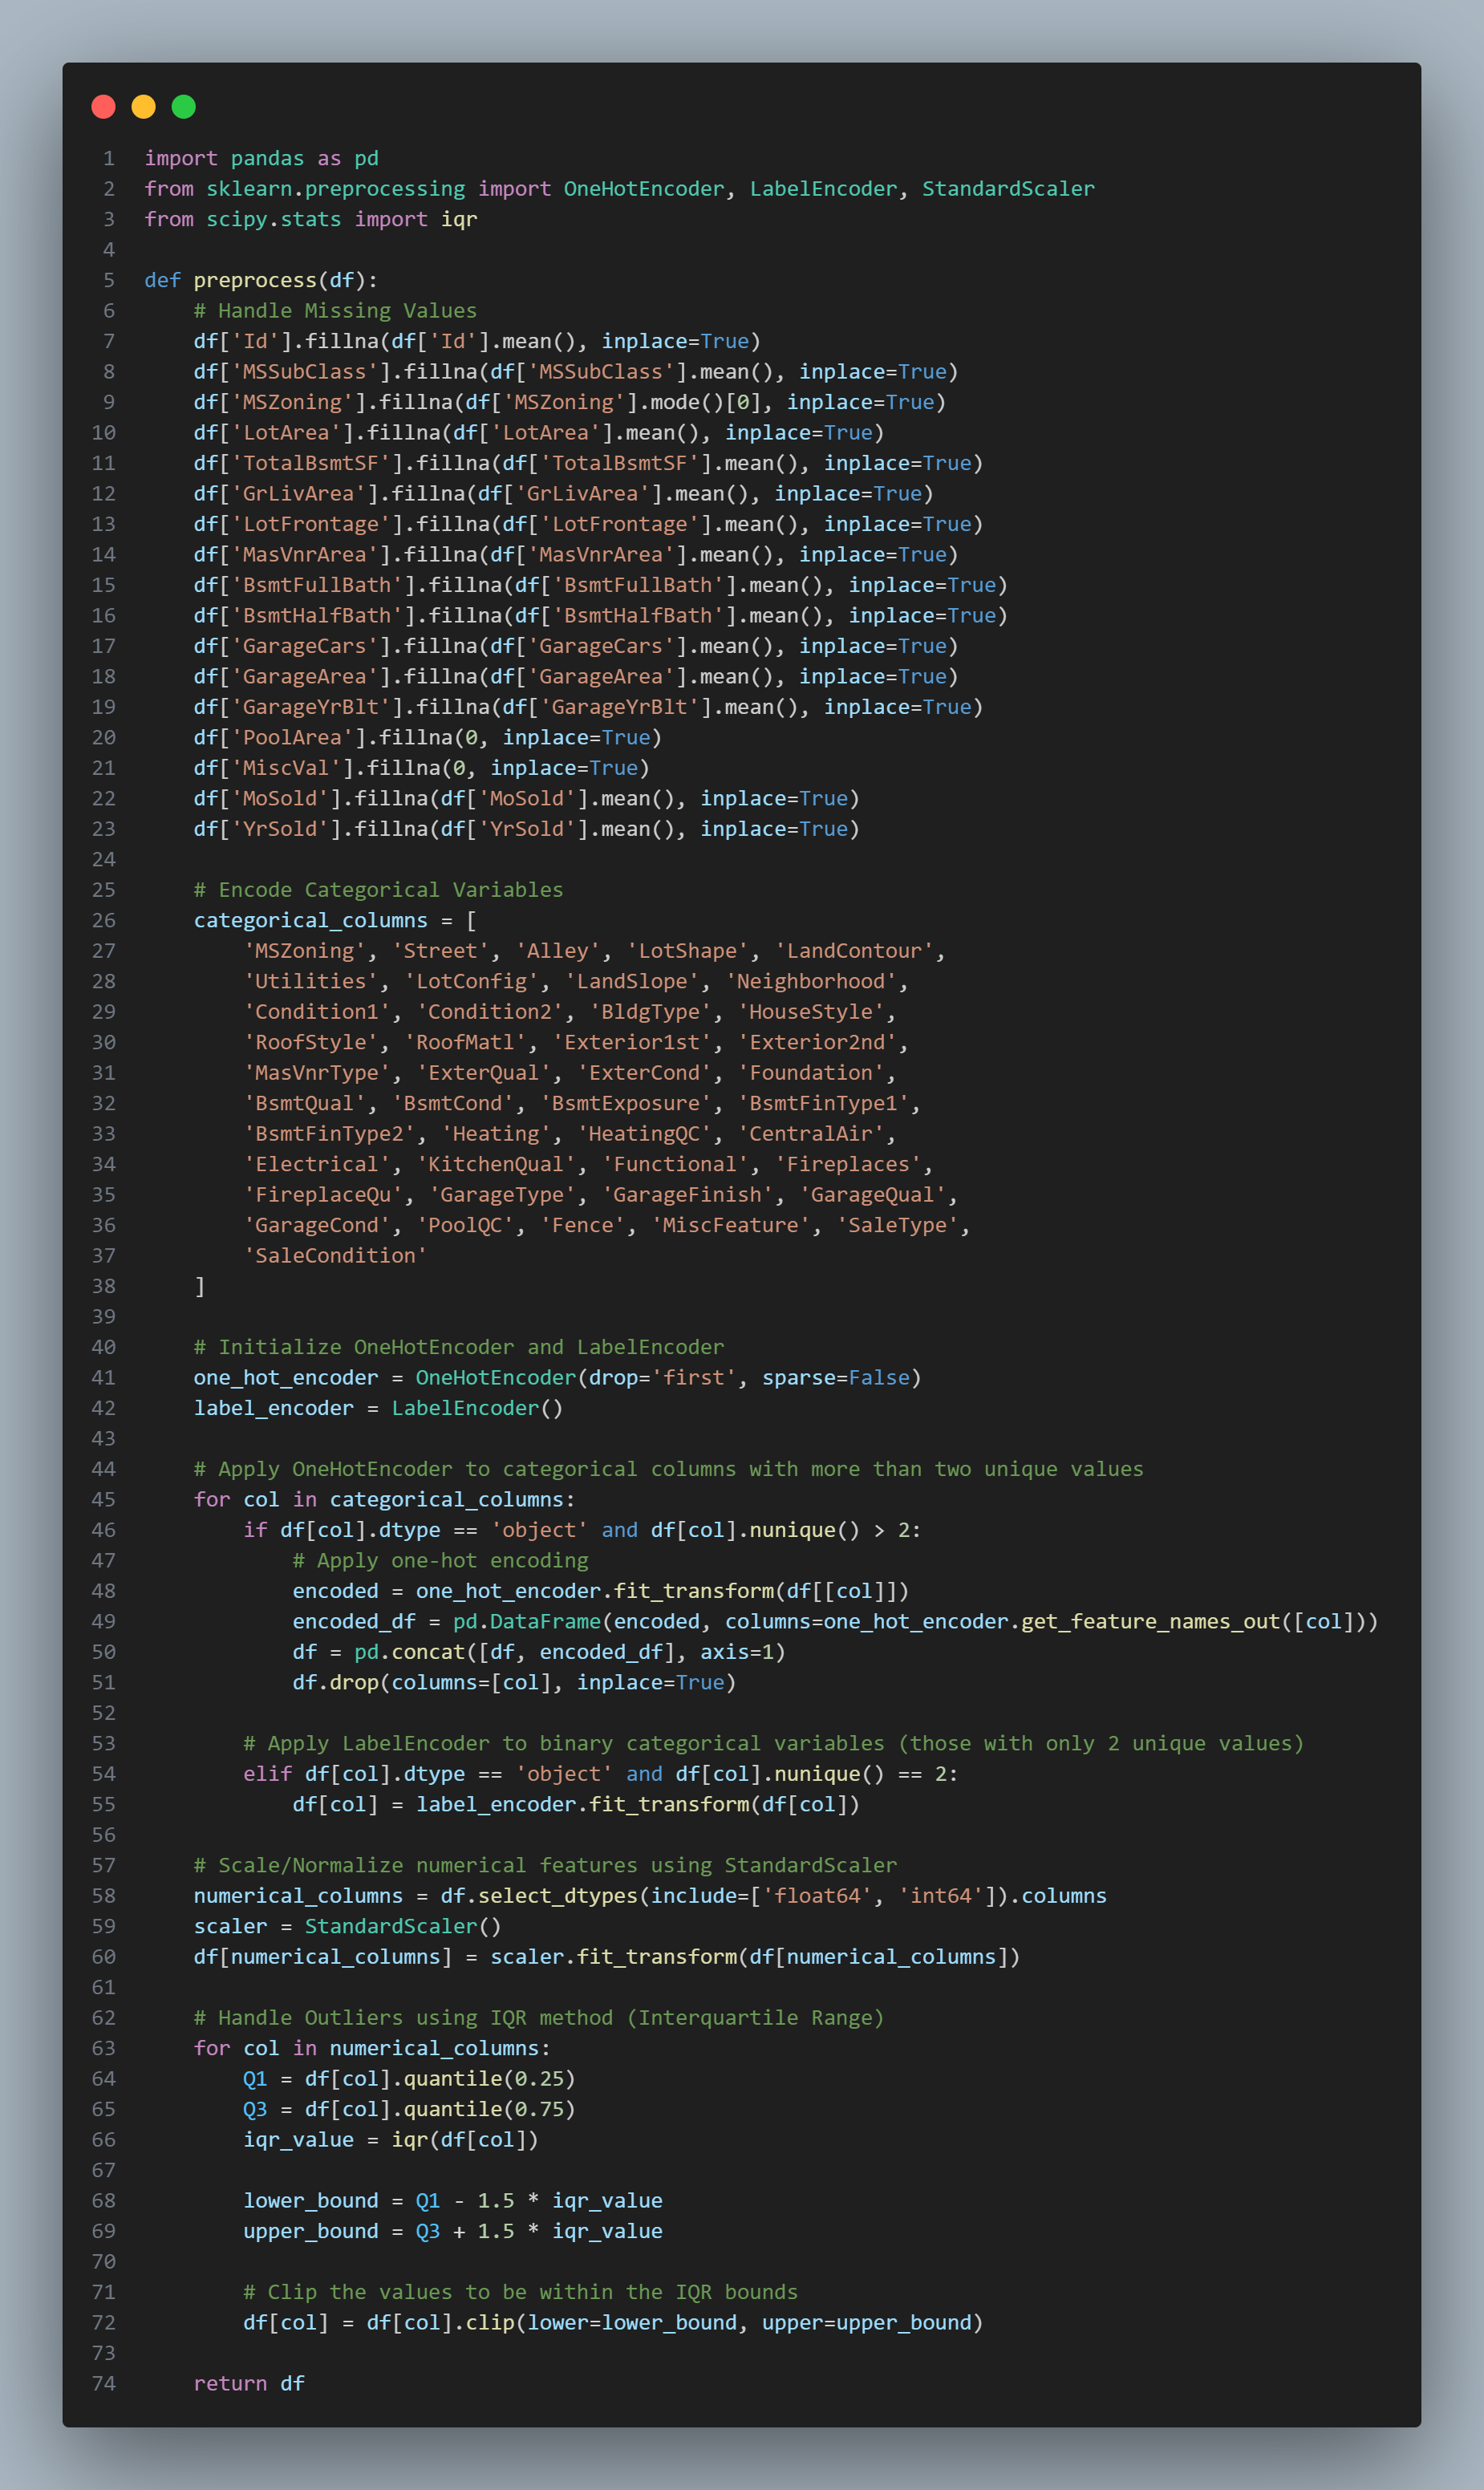
\includegraphics[width=0.9\textwidth]{media/Qwen2.5code.png}
    \caption{Example of preprocessing script generated by Qwen2.5}
    \label{fig:application-driven-preprocessing}
\end{figure}

\newpage
\subsection{Iris Dataset}

\subsubsection{Comparison 1: Preprocessing by Shoukat Khan}
This example is given by user Shoukat Khan in the following
\href{https://www.kaggle.com/code/drisrarahmad/iris-flower-dataset}{Kaggle
    link}. First thing the user did was to visualize the dataset information. After
this, the `Id' column was dropped, as it was considered unnecessary for the
future analysis of the dataset. Then some exploratory analysis was done to show
the relationships between the different features of the dataset and how they're
distributed. Then he checked the presence of null values in the dataset, but
none were found. The numerical features were then scaled using the
StandardScaler method. Finally, the dataset was split into training and testing
sets for further analysis.

\subsubsection{Comparison 2: Preprocessing by Our Team}
The Iris dataset was preprocessed by our team using a structured approach. The
dataset was loaded and examined to understand its structure and features. The
`Id' column was identified as irrelevant and removed from the dataset. The
dataset was then split into input features (X) and target variable (y). No
duplicate rows were found, so no action was taken to remove any. Missing values
were checked, but none were present in the dataset. The numerical features were
scaled using the StandardScaler method to standardize the data.

\subsubsection{Comparison 3: Preprocessing the Iris Dataset with Llama}

The Iris dataset was also preprocessed using Llama (version 3.2-Vision:11b). As
with the House Prices dataset, we provided Llama with structured prompts to
guide the preprocessing steps. However, given the relative simplicity of the
Iris dataset (with fewer features and minimal missing data) preprocessing was
more straightforward, enabling Llama to generate more accurate and usable
Python code.

For this dataset, we observed that Llama required fewer corrections compared to
the more complex House Prices dataset. The generated code effectively addressed
essential preprocessing tasks, including handling categorical data, normalizing
numerical features, and managing any missing values, though such issues were
limited in the Iris dataset.

\begin{figure}[H]
    \centering
    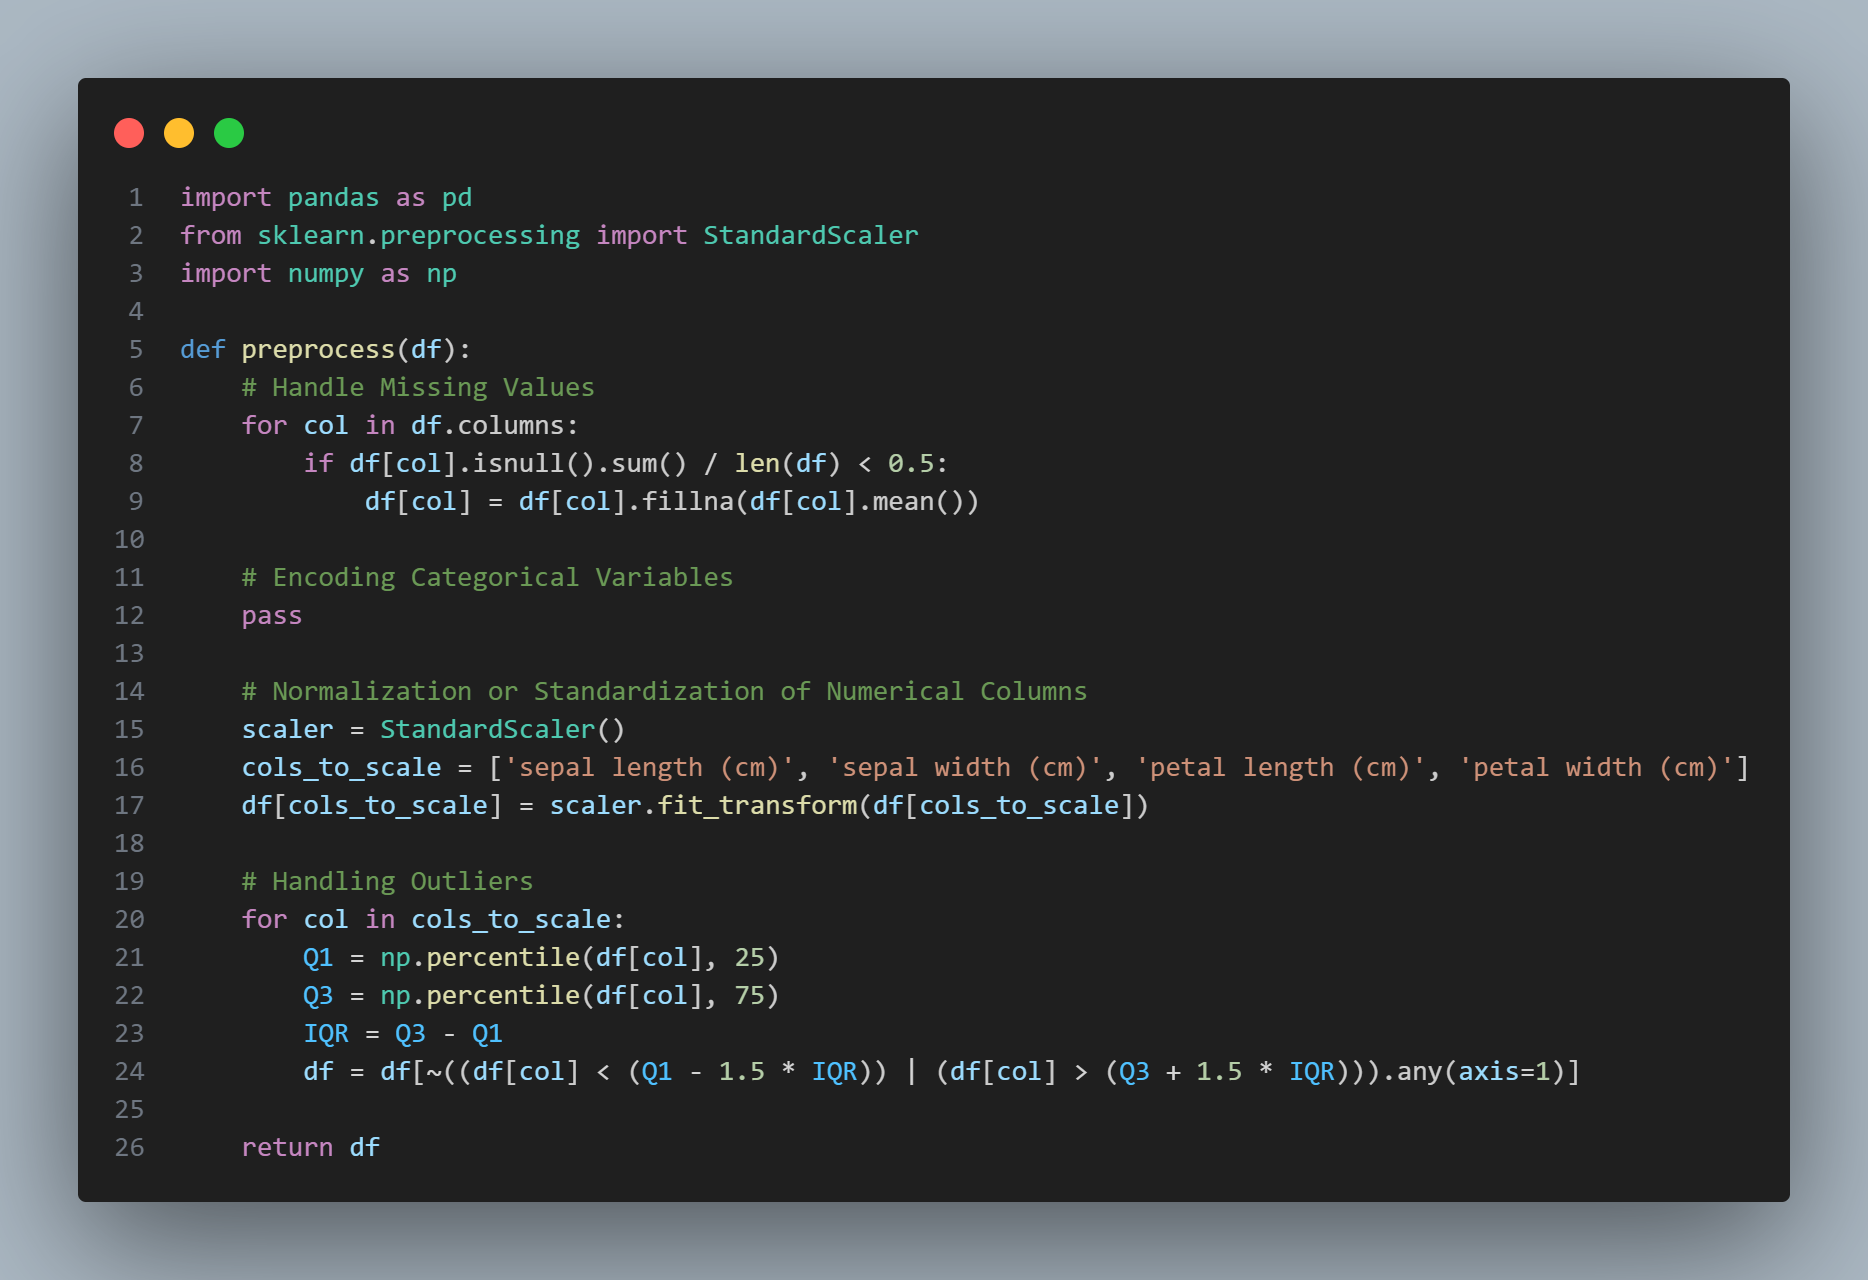
\includegraphics[width=0.7\textwidth]{media/IrisCode.png}
    \caption{Example of preprocessing script generated by LLaMA for the Iris dataset}
    \label{fig:llama-code-iris}
\end{figure}

\subsubsection{Our approach: Application-Driven Preprocessing by Qwen2.5}

Our application was also used to preprocess the Iris Dataset. Performance on
this dataset exceeded that of the House Prices dataset, which is significantly
more complex. This suggests that our application is particularly effective for
simpler datasets like Iris, while it becomes more challenging to implement on
larger and more diverse datasets.

The primary limitation lies in the model's inability to perform independent
training. Without the capability to learn autonomously, the model relies on
predictions based solely on previously observed data. Consequently, it performs
better with simpler datasets, where fewer details must be processed, allowing
for more accurate predictions. These findings indicate that the model has
considerable potential and could yield more accurate results and achieve
complete automation of data preprocessing with increased data and computational
power.

\begin{figure}[H]
    \centering
    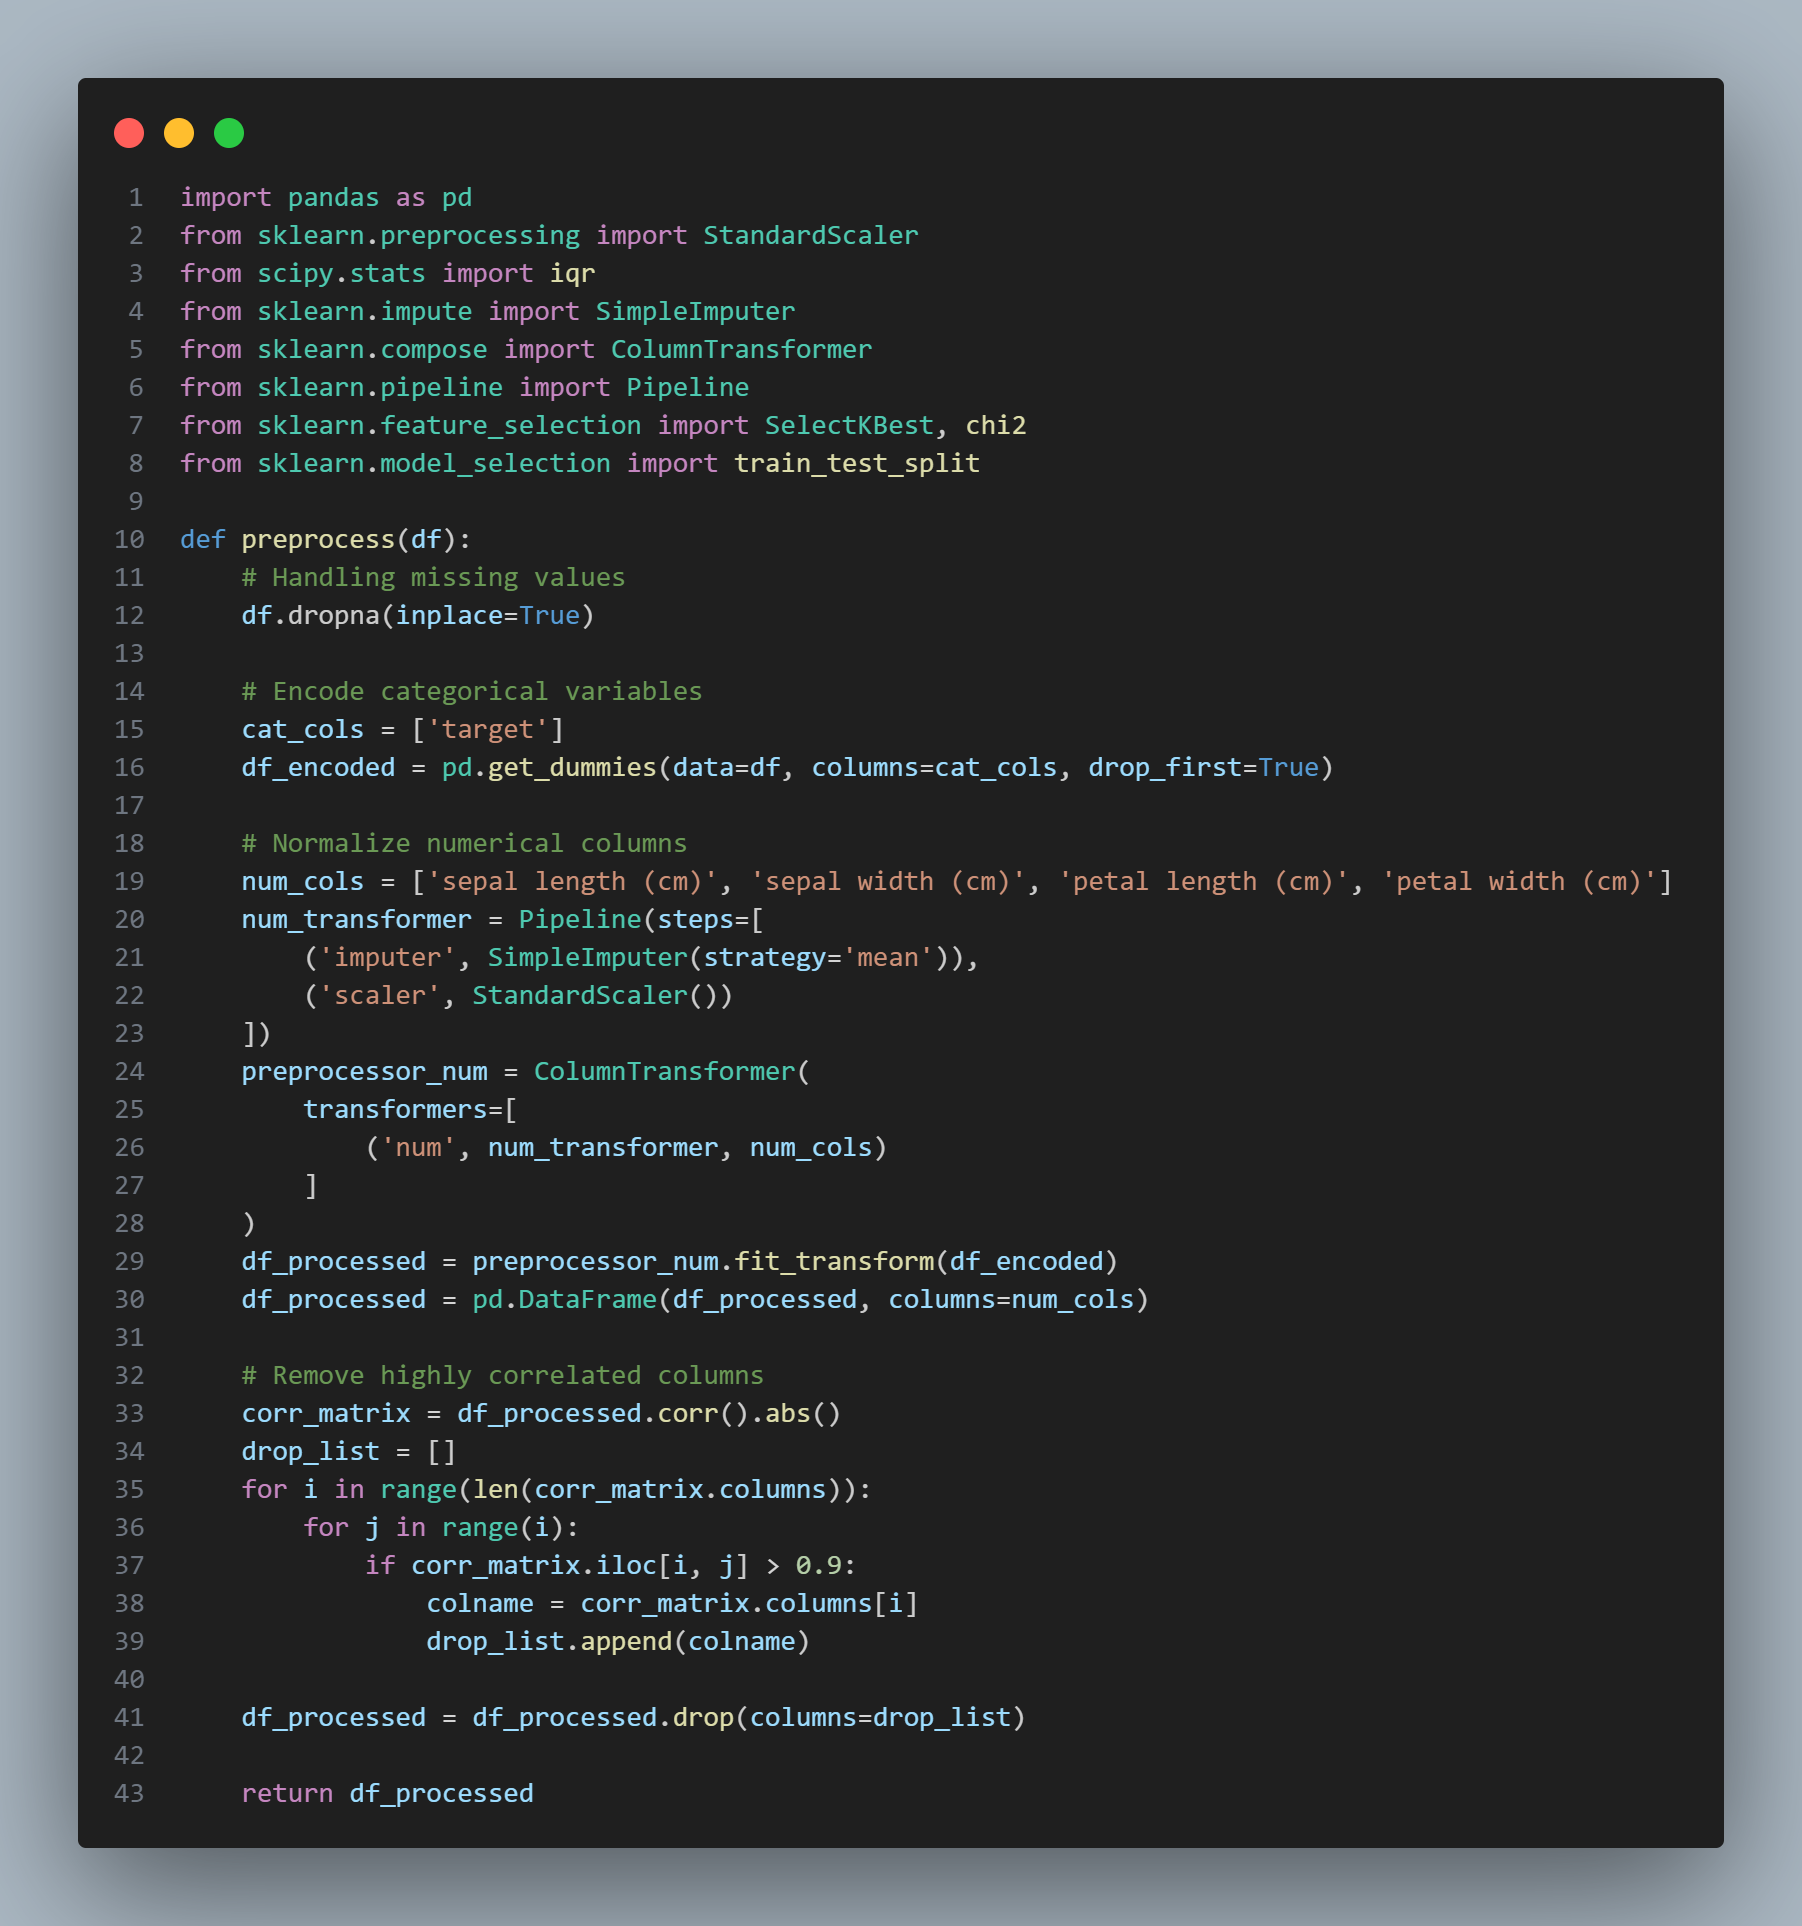
\includegraphics[width=0.7\textwidth]{media/Qwen2.5codeIRIS.png}
    \caption{Example of preprocessing script generated by Qwen2.5 for the Iris dataset}
    \label{fig:application-driven-preprocessing-iris}
\end{figure}

\subsection{Performance comparison}

% \subsubsection{House Prices Dataset}

% All the \textbf{manual approaches} carefully identify and impute missing data,
% ensuring no data loss while maintaining data integrity. Different imputation
% strategies are used based on context, with median or mean imputation for
% numerical features and domain-driven values for categorical features. They all
% transform categorical variables into numerical formats through one-hot
% encoding, label encoding, or factorization. This ensures that the data is in a
% form suitable for machine learning models. Alexandru Papiu and Erik Bruin
% emphasize encoding of ordinal features using ordinal integers when applicable,
% demonstrating consistency in preprocessing steps for such data types. Outliers
% are identified and removed, and distributions of target and input features are
% analyzed (e.g., via visual inspection). Both our team and Erik Bruin utilize
% exploratory analysis, such as plotting distributions, to better understand data
% trends and relationships between features.

% Alexandru Papiu applies a log transformation to the target variable (SalePrice)
% to reduce skewness, aligning it more closely with a normal distribution. The
% Team's approach involves standardizing numerical features using StandardScaler,
% a common practice to improve model convergence. This step was not mentioned in
% the summaries of the other manual approaches but remains a potential
% consideration for enhancing the comparability of numeric inputs.\\

% Both \textbf{AI-driven approaches} involve automated code generation based on
% input prompts, leveraging the capabilities of large language models (LLMs) to
% understand and perform preprocessing tasks. The use of role prompting in LLaMA
% guides it to generate tailored responses, demonstrating the value of carefully
% constructed prompts in directing AI behavior.

% The AI approaches automate typical preprocessing tasks such as imputation,
% normalization, and encoding of categorical variables. The focus on basic data
% cleaning, normalization, and transforming features for compatibility with
% machine learning models shows their potential to streamline preprocessing
% tasks.\\

% Manual approaches demonstrate a nuanced understanding of data context. For
% example, Erik Bruin groups related features for handling (e.g., Pool, Garage,
% and Basement), applies specific imputation strategies based on domain
% knowledge, and tailors transformations according to feature distributions.
% AI-driven methods tend to follow generalized rules or learned heuristics, which
% may not account for specific domain considerations without further tuning and
% guidance.

% Manual methods allow for fine-tuning based on data insights gained from
% exploration, such as identifying and removing outliers, specific imputation
% strategies, and encoding schemes tailored to data distributions. AI-driven
% methods like LLaMA often require human intervention to refine the generated
% code, demonstrating limitations in achieving optimal solutions without manual
% oversight.

% AI approaches offer a faster, automated process for generating initial
% preprocessing scripts, reducing the amount of repetitive work required by data
% scientists. This can be highly beneficial for rapid prototyping. Manual
% approaches are more time-consuming but can be more precise due to direct human
% involvement and domain knowledge.

% Manual methods generally exhibit fewer errors because they leverage human expertise to identify and address issues during each preprocessing step. In contrast, AI-driven preprocessing, such as that performed by Qwen2.5, often produces code that can be suboptimal or contain errors without substantial human refinement. In our experiment, the LLM's output was often insufficiently accurate, remaining overly generic and requiring numerous iterations to yield a functional solution. Even then, the results fell short of the quality expected for reliable preprocessing. This highlighted a significant gap in the model's ability to autonomously make effective decisions, underscoring the need for substantial improvement before it can be considered a viable alternative to human-led preprocessing in complex scenarios.

% \begin{figure}[H]
%     \centering
%     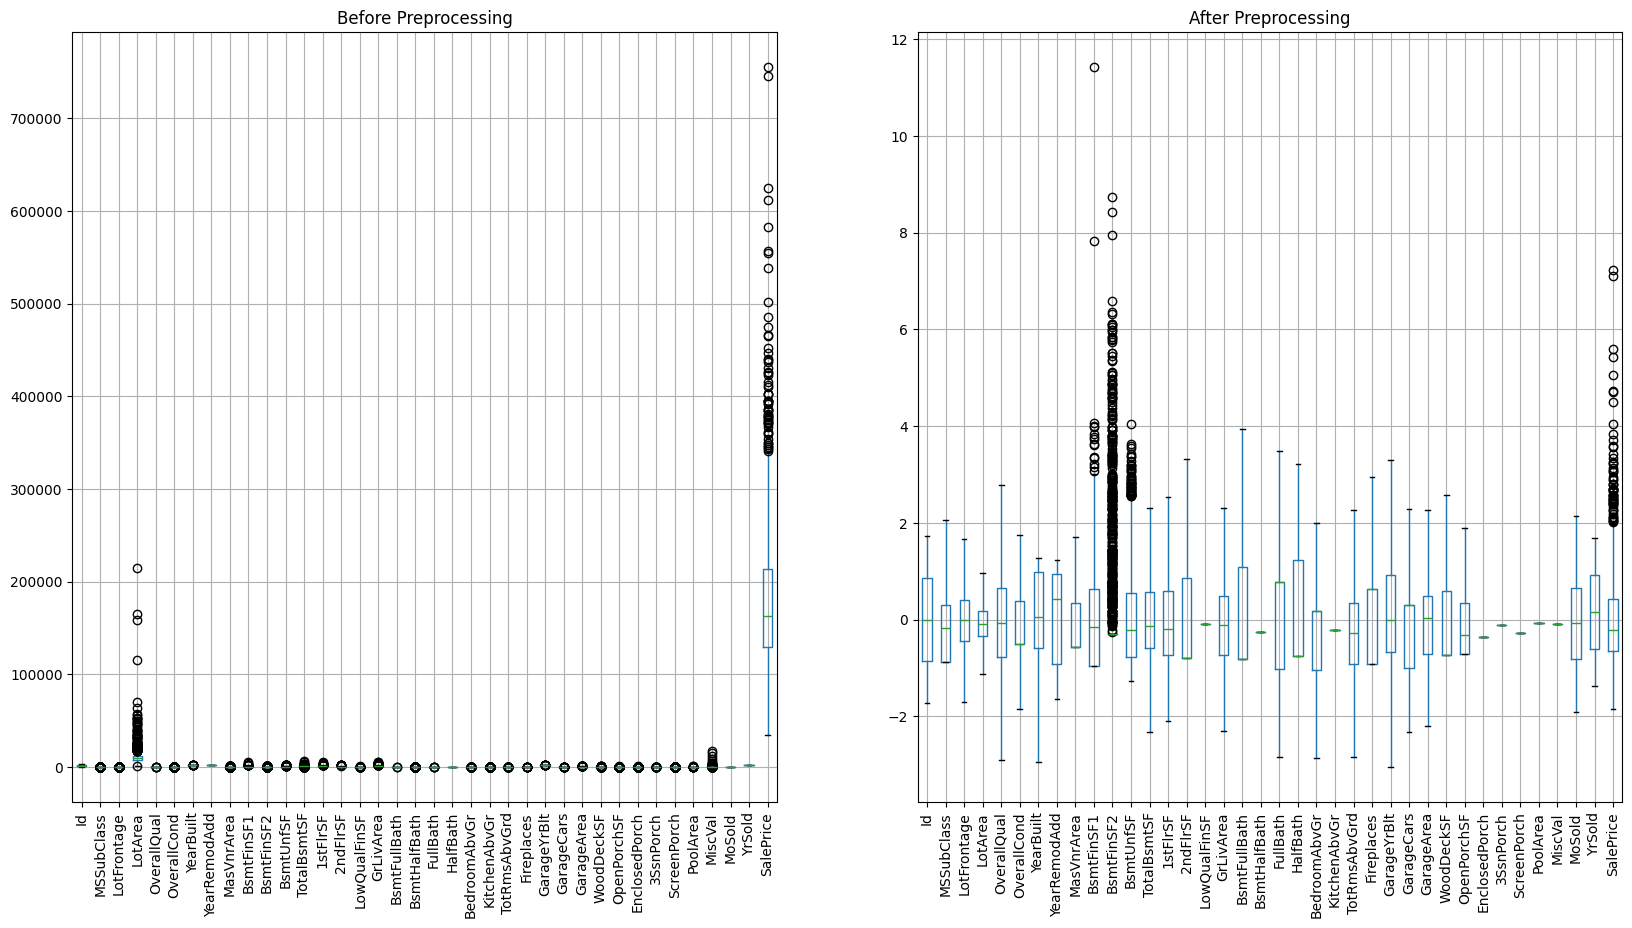
\includegraphics[width=1\textwidth]{media/comparison_house_prices.png}
%     \caption{Visualization of the data distribution before and after preprocessing}\label{fig:comparison-house-prices}
% \end{figure}

% \subsubsection{Iris Dataset}
% For the \textbf{manual approaches}, both the one by Shoukat Khan and our team
% started by loading the dataset, dropping the 'Id' column, and checking for null
% values and duplicates (with no duplicates or missing values found). This
% indicates a methodical approach to data cleaning. They used the StandardScaler
% method to scale numerical features, ensuring that data was standardized before
% applying any models. Both methods split the dataset into training and testing
% sets for further analysis, suggesting a consistent emphasis on validating model
% performance.\\ 
% The \textbf{AI-Driven Approaches} (Llama-based and
% application-driven ones) relied heavily on automation, which made preprocessing
% faster and consistent. Despite the simplicity of the Iris dataset, they
% effectively handled essential preprocessing steps, such as normalization and
% addressing potential issues like missing data (even though minimal issues were
% present). Both approaches excelled with simpler datasets like the Iris dataset,
% indicating that their strength lies in handling routine preprocessing tasks
% efficiently without much need for human intervention.\\ 
% In conclusion, manual
% approaches offered greater control and flexibility, allowing for a deeper
% understanding of the data, exploratory analysis, and custom preprocessing
% steps. On the other hand, the AI-driven methods focused on automating tasks to
% save time and reduce human effort, at the expense of adaptability and tailored
% transformations. In fact, manual methods are better suited to more complex data
% scenarios, as they allow for customization and tailored adjustments based on
% data insights, while AI-driven methods may be less flexible, especially for
% edge cases, and often require human oversight when facing unexpected data
% patterns.

% \begin{figure}[H]
%     \centering
%     \includegraphics[width=1\textwidth]{media/comparison_iris.jpg}
%     \caption{Visualization of the data distribution before and after preprocessing}\label{fig:comparison-iris}
% \end{figure}

\subsubsection{House Prices Dataset}

All the \textbf{manual approaches} carefully identify and impute missing data,
ensuring no data loss while maintaining data integrity. Different imputation
strategies are used based on context, with median or mean imputation for
numerical features and domain-driven values for categorical features. They all
transform categorical variables into numerical formats through one-hot
encoding, label encoding, or factorization. This ensures that the data is in a
form suitable for machine learning models. Alexandru Papiu and Erik Bruin
emphasize encoding of ordinal features using ordinal integers when applicable,
demonstrating consistency in preprocessing steps for such data types. Outliers
are identified and removed, and distributions of target and input features are
analyzed (e.g., via visual inspection). Both our team and Erik Bruin utilize
exploratory analysis, such as plotting distributions, to better understand data
trends and relationships between features.

Alexandru Papiu applies a log transformation to the target variable (SalePrice)
to reduce skewness, aligning it more closely with a normal distribution. The
Team's approach involves standardizing numerical features using StandardScaler,
a common practice to improve model convergence. This step was not mentioned in
the summaries of the other manual approaches but remains a potential
consideration for enhancing the comparability of numeric inputs.\\

Both \textbf{AI-driven approaches} involve automated code generation based on
input prompts, leveraging the capabilities of large language models (LLMs) to
understand and perform preprocessing tasks. The use of role prompting in Qwen2.5
guides it to generate tailored responses, demonstrating the value of carefully
constructed prompts in directing AI behavior.

The AI approaches automate typical preprocessing tasks such as imputation,
normalization, and encoding of categorical variables. The focus on basic data
cleaning, normalization, and transforming features for compatibility with
machine learning models shows their potential to streamline preprocessing
tasks.\\

Manual approaches demonstrate a nuanced understanding of data context. For
example, Erik Bruin groups related features for handling (e.g., Pool, Garage,
and Basement), applies specific imputation strategies based on domain
knowledge, and tailors transformations according to feature distributions.
AI-driven methods tend to follow generalized rules or learned heuristics, which
may not account for specific domain considerations without further tuning and
guidance.

Manual methods allow for fine-tuning based on data insights gained from
exploration, such as identifying and removing outliers, specific imputation
strategies, and encoding schemes tailored to data distributions. AI-driven
methods using Qwen2.5 and LLaMA often require human intervention to refine the generated
code, demonstrating limitations in achieving optimal solutions without manual
oversight.

AI approaches offer a faster, automated process for generating initial
preprocessing scripts, reducing the amount of repetitive work required by data
scientists. This can be highly beneficial for rapid prototyping. Manual
approaches are more time-consuming but can be more precise due to direct human
involvement and domain knowledge.

Manual methods generally exhibit fewer errors because they leverage human expertise to identify and address issues during each preprocessing step. In contrast, AI-driven preprocessing, such as that performed by Qwen2.5, often produces code that can be suboptimal or contain errors without substantial human refinement. In our experiment, the LLM's output was often insufficiently accurate, remaining overly generic and requiring numerous iterations to yield a functional solution. Even then, the results fell short of the quality expected for reliable preprocessing. This highlighted a significant gap in the model's ability to autonomously make effective decisions, underscoring the need for substantial improvement before it can be considered a viable alternative to human-led preprocessing in complex scenarios.

\begin{figure}[H]
    \centering
    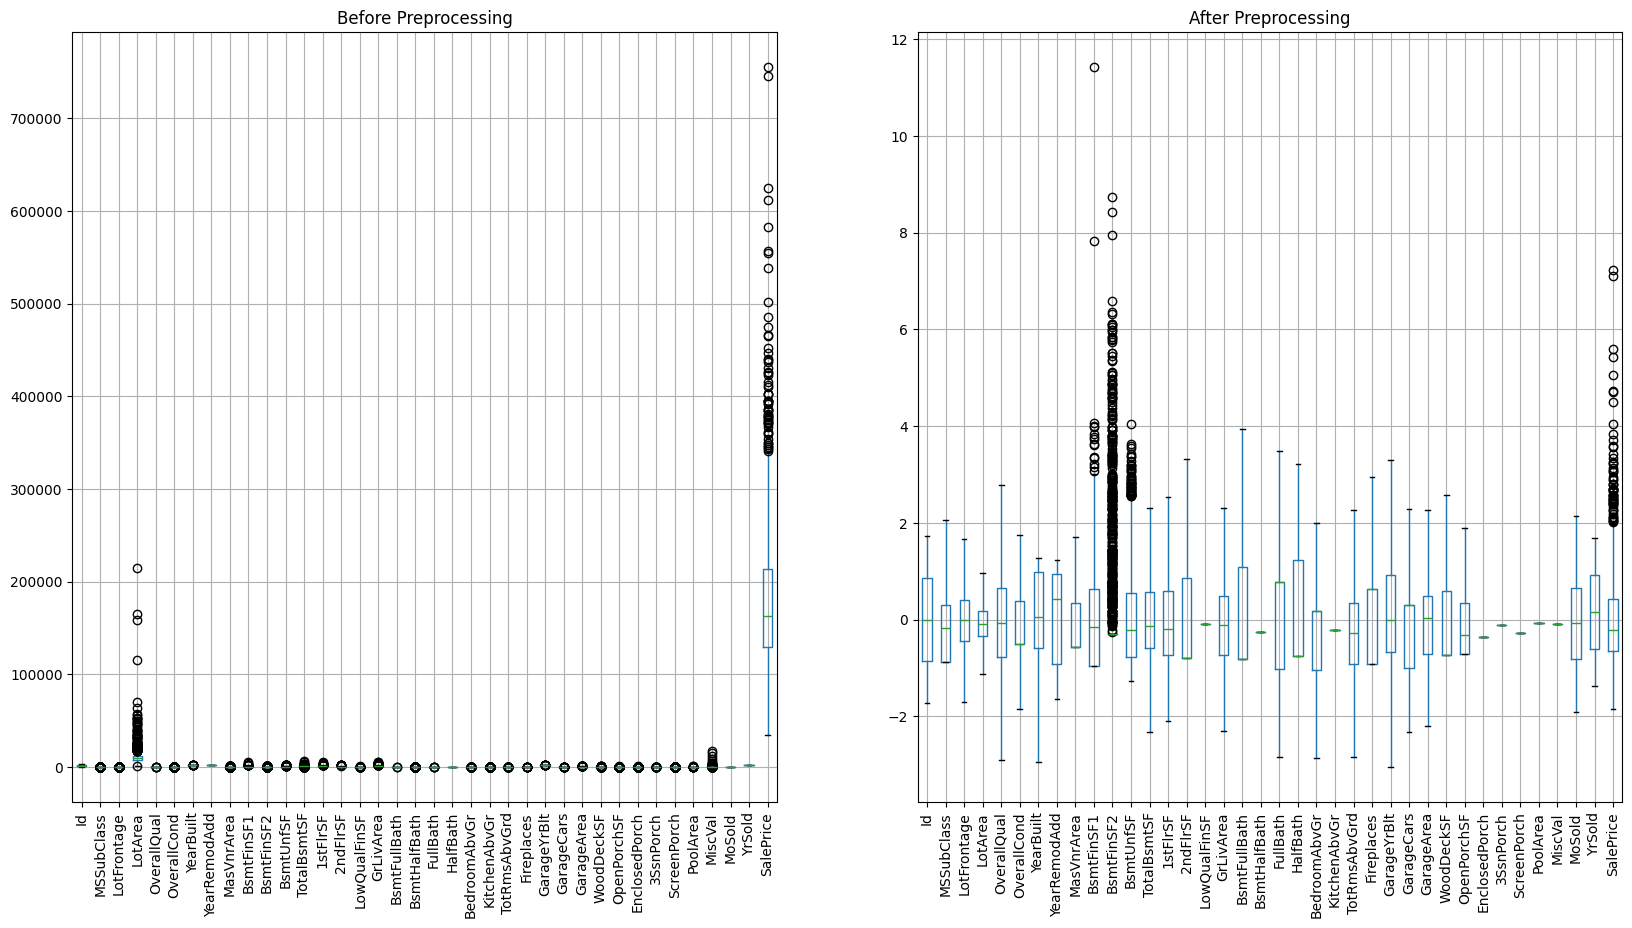
\includegraphics[width=1\textwidth]{media/comparison_house_prices.png}
    \caption{Visualization of the data distribution before and after preprocessing}\label{fig:comparison-house-prices}
\end{figure}

\subsubsection{Iris Dataset}
For the \textbf{manual approaches}, both the one by Shoukat Khan and our team
started by loading the dataset, dropping the 'Id' column, and checking for null
values and duplicates (with no duplicates or missing values found). This
indicates a methodical approach to data cleaning. They used the StandardScaler
method to scale numerical features, ensuring that data was standardized before
applying any models. Both methods split the dataset into training and testing
sets for further analysis, suggesting a consistent emphasis on validating model
performance.\\ 
The \textbf{AI-Driven Approaches} (Qwen2.5 and Llama-based) 
relied heavily on automation, which made preprocessing faster and 
consistent. Despite the simplicity of the Iris dataset, they
effectively handled essential preprocessing steps, such as normalization and
addressing potential issues like missing data (even though minimal issues were
present). Both approaches excelled with simpler datasets like the Iris dataset,
indicating that their strength lies in handling routine preprocessing tasks
efficiently without much need for human intervention.\\ 
In conclusion, manual
approaches offered greater control and flexibility, allowing for a deeper
understanding of the data, exploratory analysis, and custom preprocessing
steps. On the other hand, the AI-driven methods focused on automating tasks to
save time and reduce human effort, at the expense of adaptability and tailored
transformations. In fact, manual methods are better suited to more complex data
scenarios, as they allow for customization and tailored adjustments based on
data insights, while AI-driven methods may be less flexible, especially for
edge cases, and often require human oversight when facing unexpected data
patterns.

\begin{figure}[H]
    \centering
    \includegraphics[width=1\textwidth]{media/comparison_iris.jpg}
    \caption{Visualization of the data distribution before and after preprocessing}\label{fig:comparison-iris}
\end{figure}